% Pursuing Stacks (cotes 134-2 to 134-8): archive cote 134-3, site page 60 (PDF page 61), typescript page 60.
% typescript. Draft compared: ps2.tex:3049-3123.
% AI-transcribed by Claude Opus 5.5 (claude-opus-5-5, adaptive thinking, effort high), Message Batches API, batch ps1 (msgbatch_01Rv5hCaNTtUt4JHx1yqoHPL), 2026-11-12; image review recorded in records/CHECK_DECISIONS_134_3_4.tsv.
\scanpage{134-3/60}
\mspage{\hand{60}}

We now get the (essentially trivial)
\uline{Homotopy lemma} \ Let \ $h\colon FxI \hand{\longrightarrow} F$ be a ``homotopy'' with respect to $(I,e_o,e_1)$
of $\mathrm{id}_F$ \ with a constant map \xout{ix} $c = ir\colon F \hand{\to} F$ , \ where $r\colon F \hand{\longrightarrow} e$ and \xout{i}
$i\colon e \hand{\to} F$ is a section of $F$ over $e$. \ Then $F \hand{\to} e$ is \ W-aspheric.

In the proof of this lemma, \ we make use of a)b)c) for W, \ but only
of a)c) for $(I,e_o,e_1)$ \ namely we don't even need \ $e_o \hand{\cap} e_1 = \hand{\emptyset}_{\hand{\mathcal{A}}}$ . \ This is
\inserted[typed]{still the case for} \xout{property however will be used in} the proof of the
\uline{Comparison lemma for homotopy intervals}: \ Let L be an object of \hand{\ensuremath{\mathcal{A}}} , squa-%
rable over e and endowed with a composition law \ $x\hand{\wedge}y$ ; \ let \ $\over{e}{\delta}_i^L \colon e \hand{\to} L$
be two sections of L (i \hand{\ensuremath{\in\{}}0,1\hand{\ensuremath{\}}} ), \ which are respectively a left unit and a
zero element for the multiplication,namely the corresponding elements
$\hand{e}_o^{\over[typed]{\illegible{1}}{a}},\hand{e}_1^{\over[typed]{\illegible{1}}{a}}$ \ in any Hom(\over[typed]{\illegible{1}}{a},L) satisfy
\[ \hand{e}_{\over{\unsure{o}}{1}}^{\over[typed]{\illegible{1}}{a}} \hand{\wedge} x = x \ , \ \hand{e}_{\over{\unsure{1}}{0}}^{\over[typed]{\illegible{1}}{a}} \hand{\wedge} x \ = \hand{e}_{\over{\unsure{1}}{0}}^{\over[typed]{\illegible{1}}{a}} \]
for any x in Hom(\over[typed]{\illegible{1}}{a},L). \ Assume moreover we got a homotopy interval $(I,e_o,$
$e_1)$ and a \hand{``}map of intervals\hand{''}
\[ \hand{\phi}\colon I \hand{\longrightarrow} L \]
(in the sense: \ compatible with endpoints). \ Then \ $\mathrm{id}_L$ is homotopic(with
respect to $(I,e_o,e_1)$) to the constant map $c_{\hand{\unsure{0|a}}}\colon L \hand{\to} L$ defined by $\hand{\delta}^L_{\hand{\unsure{0|a}}}$ , \ and
hence by the previous homotopy lemma, \ $L \hand{\to} e$ is W-aspheric and therefore
\xout{\illegible{1}} L endowed with \ $e_o^L ,e_1^L$ \ defined by $\hand{\delta}_o^L,\hand{\delta}_1^L$ \ is itself a homotopy inter-%
val in \hand{\ensuremath{\mathcal{A}}} (provided, \ at least, we know \ that \ $e_o^L \hand{\cap} e_1^L = \hand{\emptyset}$ ).

The homotopy h is simply given \ (for \ $u\colon \over[typed]{\illegible{1}}{a} \hand{\to} \over[typed]{\illegible{1}}{I}$, \ $x\colon \over[typed]{\illegible{1}}{a} \hand{\to} L$) by
\[ h(\over[typed]{\illegible{1}}{x},\over[typed]{\illegible{1}}{u}) = \xout{uxxxxx} \ \hand{\phi}(u) \hand{\wedge} x \ , \]
when a factors through $e_{\hand{1}}$ then $\hand{\phi}(u) = \hand{e}^a_{\hand{1}}$ \ and hence \ $h(x,u)=x$, \ if it
factors through $e_{\hand{0}}$ then $\hand{\phi}(u) = \hand{e}^a_{\hand{0}}$ \ and we get $h(x,u) = \hand{e}^a_{\hand{0}}$ , \ qed.
\uline{Corollary} \ Assume in \hand{\ensuremath{\mathcal{A}}} (endowed with W) finite inverse limits exist
(i.e. final object and fibered products exist), \ and moreover that the
\deleted{functor}\inserted{presheaf} \hand{on $\mathcal{A}$}
\[ F \hand{\longmapsto} \text{set ob all subobjects of } F \]
is representable by an element L of \hand{\ensuremath{\mathcal{A}}} (the ``Lawvere element''). \ \xout{Then}
Assume moreover \hand{\ensuremath{\mathcal{A}}} has a\xout{n} strict initia\over[typed]{\unsure{b}}{l} element $\hand{\emptyset}_{\hand{\mathcal{A}}}$, i.e. an initial
element and that \deleted{\xout{for}} any \ map \ $\underset{\text{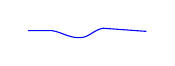
\begin{tikzpicture}[x=1cm,y=1cm,baseline]\draw[color=blue] (0,0.05)--(0.3,0.05) to[out=-10,in=180] (0.65,-0.04) to[out=0,in=190] (0.95,0.08)--(1.5,0.04);\end{tikzpicture}}}{a \hand{\to} \hand{\emptyset}_{\hand{\mathcal{A}}}}$ \ is an isomorphism. \ Consider the
two sections of L over e , $\hand{\delta}^L_{\hand{1}}$ \ and \ $\hand{\delta}^L_{\hand{0}}$ , \ corresponding to the full and
to the empty subobject of e, \ so that we get visibly \ $e_o^L \hand{\cap} e_1^L = \hand{\emptyset}$ \ .
\over{t}{T}hen, \ for a homotopy interval to exist in \hand{\ensuremath{\mathcal{A}}} , it is necessay and suf-%
ficient that L be W-aspheric over e , \ i.e. that $(L,e_o^L ,e_1^L )$ \ be a homoto-%
py interval.

By the comparison lemma, \ it is enough to show that for any homotopy
\unsure{interval} \ $(I,e_o,e_1)$ \ in \hand{\ensuremath{\mathcal{A}}}, \ there exists a morphism of ``intervals''
